\chapter{Resultados} \label{chapter:III}
\section{Scrum en la pr\'{a}ctica (1ra Iteraci\'{o}n)}
\begin{spacing}{1.5}
	\subsection{\textit{Produc BackLog}}
	Las historias fueron trabajadas en las reuniones del \textit{Scrum Team}, estuvieron presentes los \textit{Developer}, el \textit{Product Owner} y el \textit{Scrum master} y de forma b\'{a}sica empezaron a ser redactadas en los tableros de nuestro \textit{Workspace} como muestra la figura \ref{figure:chaperIII_1}.
	
	\begin{figure}[H]
		\centering
		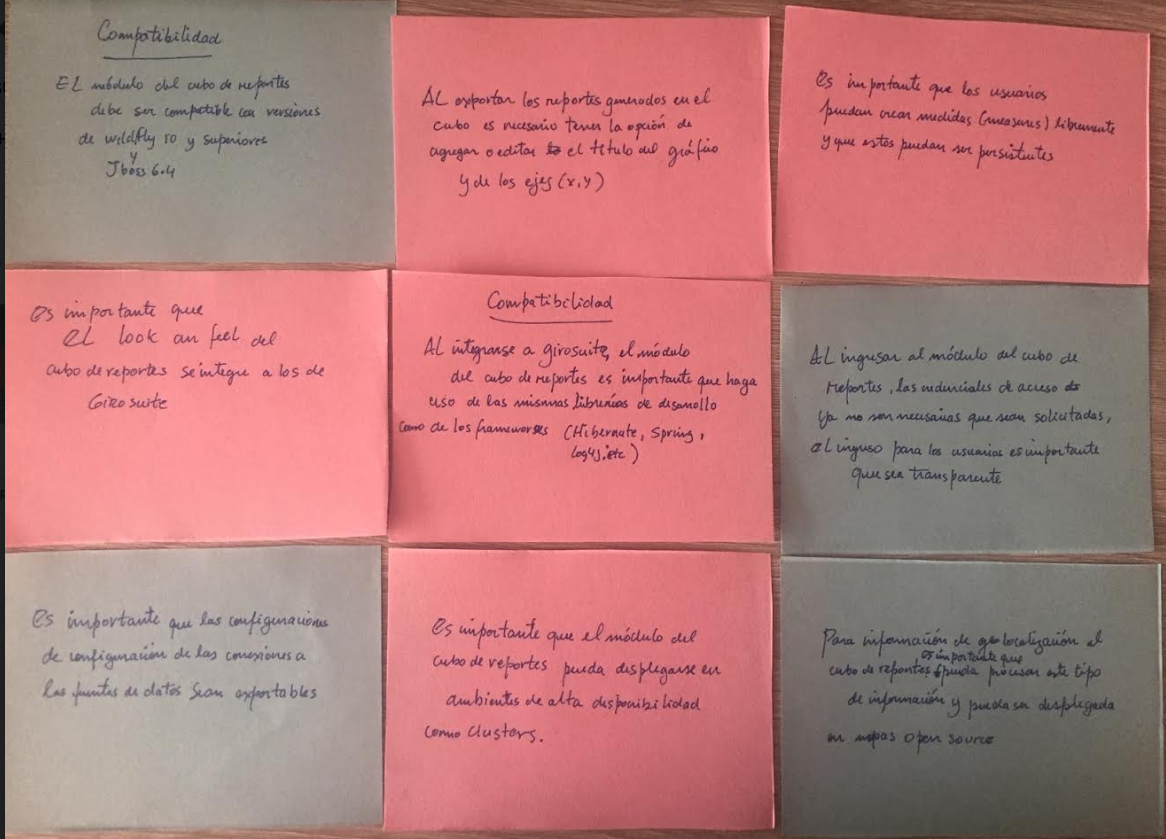
\includegraphics[width=1 \textwidth]{scrum_3_2}
		\caption {\centering \small{Product BackLog}} \label{figure:chaperIII_1}
		\small {Fuente: \'{A}rea de desarrollo de Tesla Technologies S.A.C, 2018}
	\end{figure}
	
	En la primera versi\'{o}n del \textit{Product Backlog} definieron 15 historias como l\'{i}nea base (ver figura \ref{figure:chaperIII_2}) que trataron temas de compatibilidad, escalabilidad, integraci\'{o}n y nuevas funcionalidades.

	\begin{figure}[H]
		\centering
		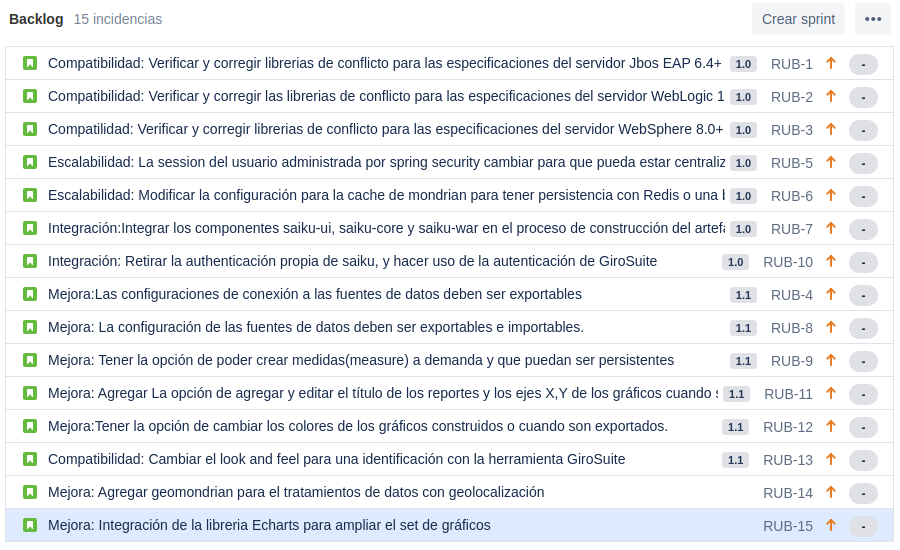
\includegraphics[width=1 \textwidth]{scrum_3_1}
		\caption {\centering \small{Product BackLog}} \label{figure:chaperIII_2}
		\small {Fuente: \'{A}rea de desarrollo de Tesla Technologies S.A.C, 2018}
	\end{figure}
	\textbf{Compromiso: Objetivo del Producto}\\
	``Integrar y mejorar las funcionalidades core de Saiku Analytics a la herramienta GiroSuite para darle potencia y din\'{a}mica a la generaci\'{o}n de reportes''\\
	
	\subsection{\textit{Sprint Planning}}
	Para establecer el trabajo que realizar\'{a} el \textit{Sprint}, el \textit{Scrum Team} debatio la propuesta del Product Owner sobre integrar las funcionalidad core del proyecto Saiku Analytics manteniendo la compatibilidad del software Giro suite con la infraestructura tecnol\'{o}gica de sus clientes; se priorizaron las siguientes historias.
	
	En el primer \textit{Sprint} se tomaron 7 historias, como se muestra en la tabla \ref{table:III_1}. 
	\begin{table}[H]\centering\small
		\begin{tabular}[H]{m{0.1\linewidth}m{0.1\linewidth}|m{0.6\linewidth} m{0.12\linewidth}}
			\hline
			\rowcolor[HTML]{CBCEFB} 
			\textbf{Tipo} & \textbf{Clave} &\textbf{Resumen} &\textbf{Estado}\\
			\hline
			Historia &RUB-10 &Integración: Retirar la autenticación propia de saiku, y hacer uso de la autenticación de GiroSuite &Tareas por hacer.\\
			\hline
			Historia &RUB-7 &Integración:Integrar los componentes saiku-ui, saiku-core y saiku-war en el proceso de construcción del artefacto de GiroSuite. &Tareas por hacer\\
			\hline
			Historia &RUB-6 &Escalabilidad: Modificar la configuración para la cache de mondrian para tener persistencia con Redis o una base de datos relacional. &Tareas por hacer\\
			\hline
			Historia &RUB-5 &Escalabilidad: La session del usuario administrada por spring security cambiar para que pueda estar centralizada en la base de datos. &Tareas por hacer\\
			\hline
			Historia &RUB-3 &Compatilidad: Verificar y corregir librerias de conflicto para las especificaciones del servidor WebSphere 8.0+ y los archivos ibm-web-bnd.xml, ibm-web-ext.xml, deployment.xml y build.properties &Tareas por hacer\\
			\hline
			Historia &RUB-2 &Compatibilidad: Verificar y corregir las librerias de conflicto para las especificaciones del servidor WebLogic 12c + y los archivos weblogic.xml y build.properties &Tareas por hacer\\
			\hline
			Historia &RUB-1 &Compatibilidad: Verificar y corregir librerias de conflicto para las especificaciones del servidor Jbos EAP 6.4+ y loss archivos jboss-deployment-structure.xml, application.xml y build.properties. &Tareas por hacer\\
			\hline
		\end{tabular}
		\caption{Historias del primer Sprint}
		\small {Fuente: \'{A}rea de desarrollo de Tesla Technologies S.A.C, 2018}
		\label{table:III_1}
	\end{table}
	\subsection{\textit{Sprint BackLog}}
		Luego de la priorizaci\'{o}n de las historias adecuerdo al compromiso del \textit{Product BackLog}, los \textit{Developers} realizamos la estimaci\'{o}n de cada historia haciendo uso de las \textit{Story Points} teniendo ya en el tablero el primer Sprint BackLog. 	
		\begin{figure}[H]
			\centering
			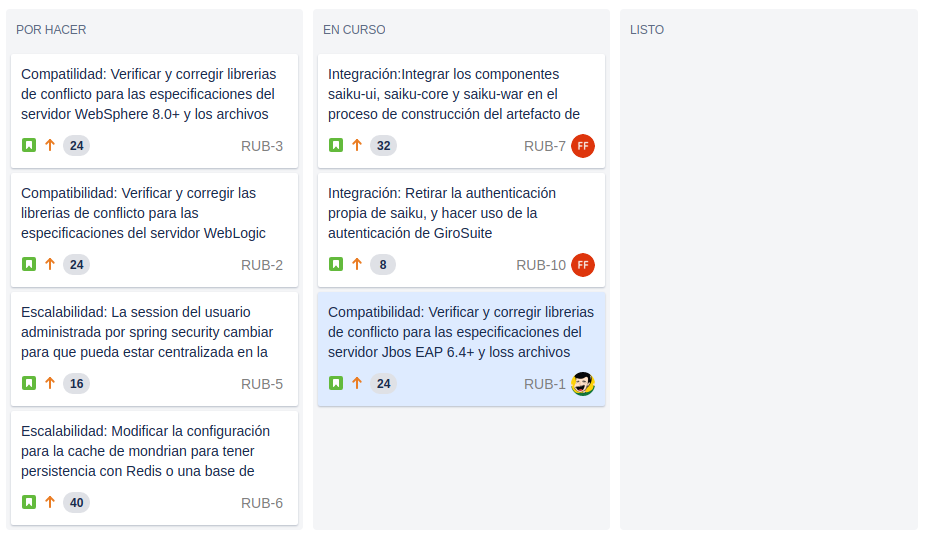
\includegraphics[width=1 \textwidth]{scrum_3_3}
			\caption {\centering \small{Sprint BackLog}} \label{figure:chaperIII_3}
			\small {Fuente: \'{A}rea de desarrollo de Tesla Technologies S.A.C, 2018}
		\end{figure}
	
		\textbf{Compromiso: Objetivo del \textit{Sprint}}\\
	``Integrar las funcionalidades core de Saiku Analytics y su compatibilidad al 100\% en la infraestructura de los clientes donde esta instalda la herramienta GiroSuite''.\\
		
	\subsection{\textit{Daily Scrum}}
		El \textit{Daily Scrum} fue una constante revisi\'{o}n del avance del proyecto, hubo reuniones que pasaron los minutos recomendados y otras no se llevaron acabo, sin embargo estas conversaciones aportaron valor al momento tomar decisiones r\'{a}pidas.
	
	\clearpage		
	\subsection{\textit{Sprint Review}}
		Analizemos el sprint review de cada historia:
		\subsubsection{Integrar los componentes saiku-ui, saiku-core y saiku-webapp, saiku-service, saiku-query, saiku-repository en el proceso de construcción del artefacto de GiroSuite.}
		
		\begin{itemize}
			\item El proyecto Saiku Analytics a nivel de fuentes correctas y compilables ya est\'{a}n descontinuadas, y se tienen sub m\'{o}dulos que no son \'{u}tiles al 100\% Figura \ref{figure:chaperIII_4}.
			
			\begin{figure}[H]
				\centering
				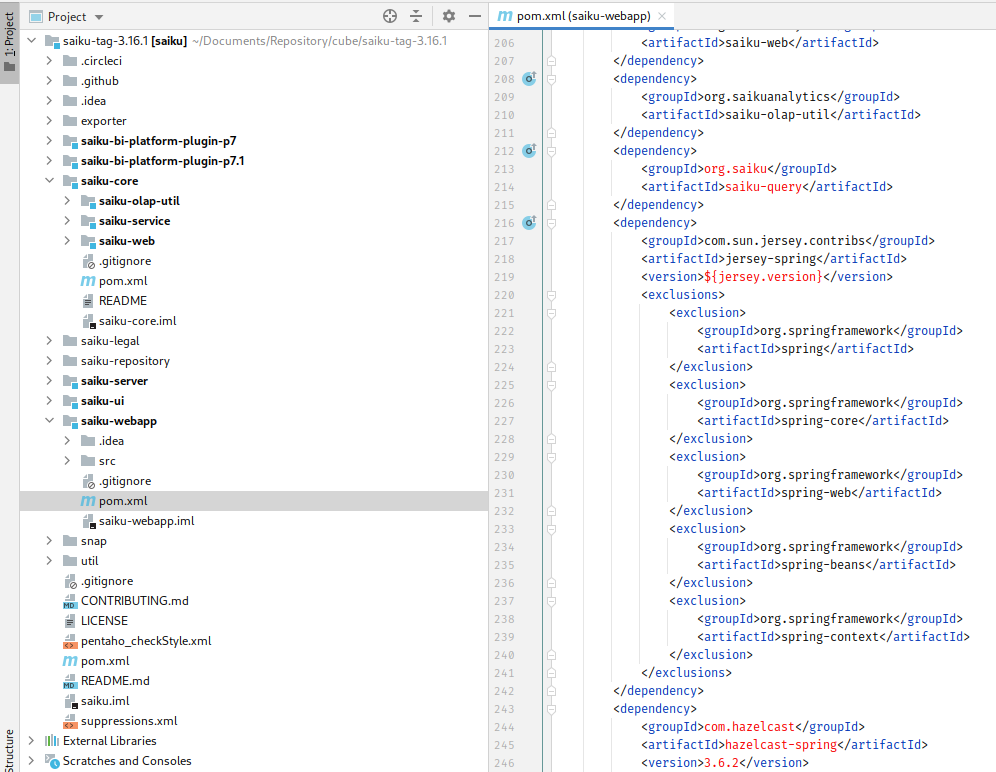
\includegraphics[width=1 \textwidth]{saiku_1}
				\caption {\centering \small{Proyecto Saiku Analytics, c\'{o}digo fuente descontinuado}} \label{figure:chaperIII_4}
				\small {Fuente: \'{A}rea de desarrollo de Tesla Technologies S.A.C, 2018}
			\end{figure}
			\item El nuevo m\'{o}dulo resultante rubik-report tiene compatibilidad al 100\% con el producto GiroSuite.
			\item El nuevo m\'{o}dulo rubik-report si contiene el c\'{o}digo fuente correcto de las funcionalidades m\'{i}nimas del proyecto Saiku Analytics ver Figura \ref{figure:chaperIII_5}.
			
			\begin{figure}[H]
				\centering
				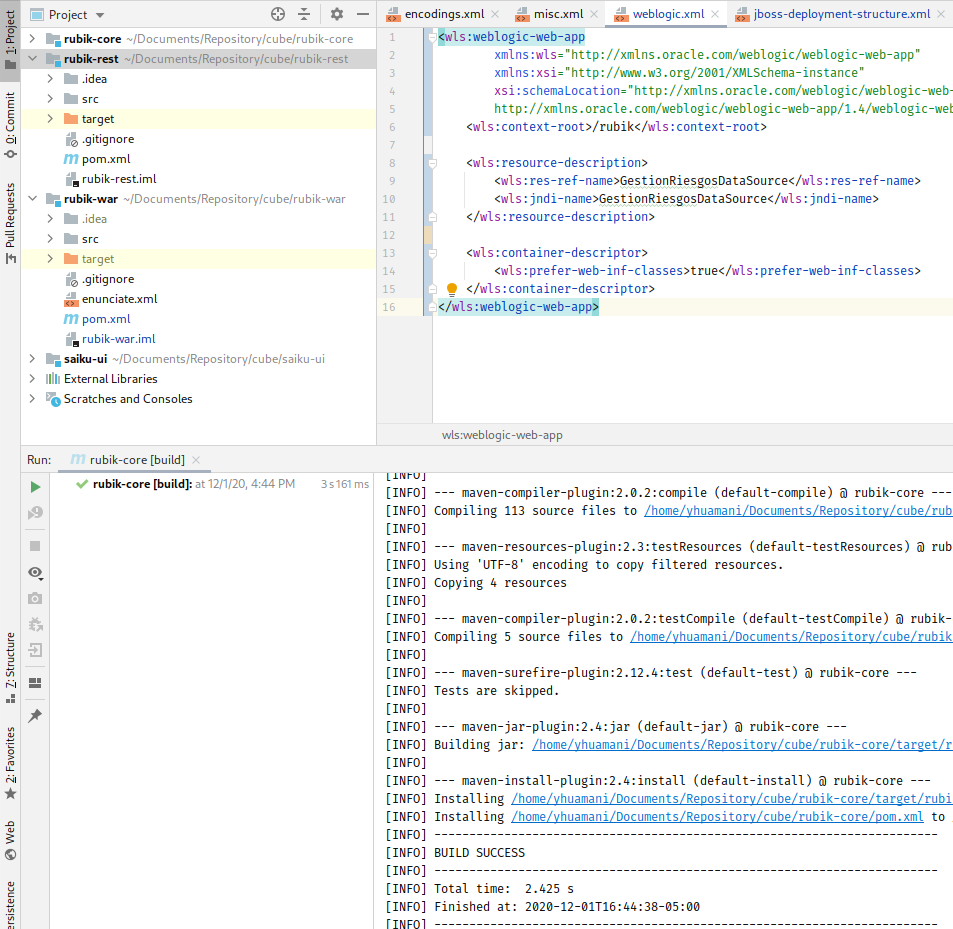
\includegraphics[width=1 \textwidth]{saiku_2}
				\caption {\centering \small{Proyecto Rubik-report, c\'{o}digo fuente}} \label{figure:chaperIII_5}
				\small {Fuente: \'{A}rea de desarrollo de Tesla Technologies S.A.C, 2018}
			\end{figure}
			
			\item El equipo recomienda reducir el n\'{u}mero de m\'{o}dulos pues 2 de ellos se encuentran ligados directamente como plugins de la Suite Pentaho Analytics.
			\item El equipo recomienda quitar todo aquello que no sea parte de la funcionalidad core y refactorizar el m\'{o}dulo rubik-query.
		\end{itemize}	
		\clearpage	
		\subsubsection{Retirar la authenticación propia de saiku, y hacer uso de la autenticación de GiroSuite}
		
		\begin{itemize}
			\item Se identifica que la Session  del usuario y la seguridad vienen configurados bajo Spring Security.
			\item Con las modificaciones puede ingresar a la aplicaci\'{o}n a travez de la herramienta GiroSuite, se implement\'{o}n, siendo transparente para el usuario ver Figura \ref{figure:chaperIII_6}.
		\end{itemize}
		
		\begin{figure}[H]
			\centering
			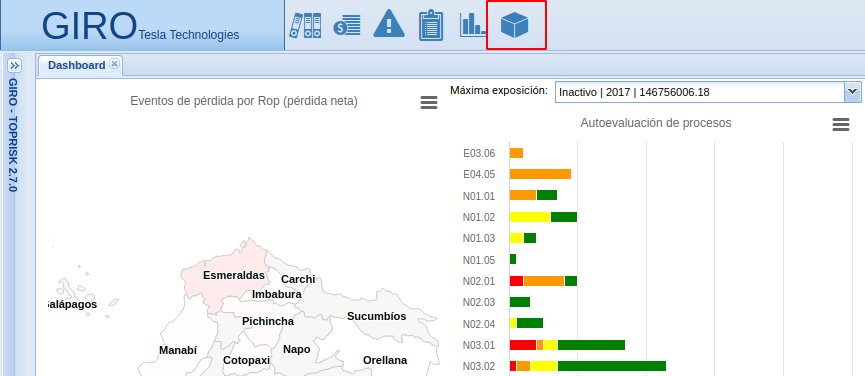
\includegraphics[width=1 \textwidth]{saiku_3}
			\caption {\centering \small{Proyecto Rubik-report integrado a GiroSuite}} \label{figure:chaperIII_6}
			\small {Fuente: \'{A}rea de desarrollo de Tesla Technologies S.A.C, 2018}
		\end{figure}	
			
		\subsubsection{Compatibilidad: Verificar y corregir librerias de conflicto para las especificaciones del servidor Jbos EAP 6.4+ y loss archivos jboss-deployment-structure.xml, application.xml y build.properties.}
		
		\begin{itemize}
			\item En la verificaci\'{o}n de los clientes se encontraron conflictos con las version Jbos EAP 6.4, 7.0 y sus versiones comunitarias Wildfly 10.0 Final, 10.1 y 11.0.
			\item Los conflictos son por configuraciones internas de los cliente como jasper reports 3.0, implementaciones del standard JPA 1.0, spring framework 2.5, librerias de JAX-WS.
			\item El equipo recomienda mantenerse en la JRS-366(Jdk 8) y eso debe comunicarse al equipo de ventas para no modificar esta especificaci\'{o}n.
			\item Actualmente GiroSuite ya integrado con Rubik Report puede desplegar en las versiones Jbos EAP 6.4, 7.0 y sus versiones comunitarias Wildfly 10.0 Final, 10.1 y 11.0, ver Figura \ref{figure:chaperIII_7}
			\begin{figure}[H]
				\centering
				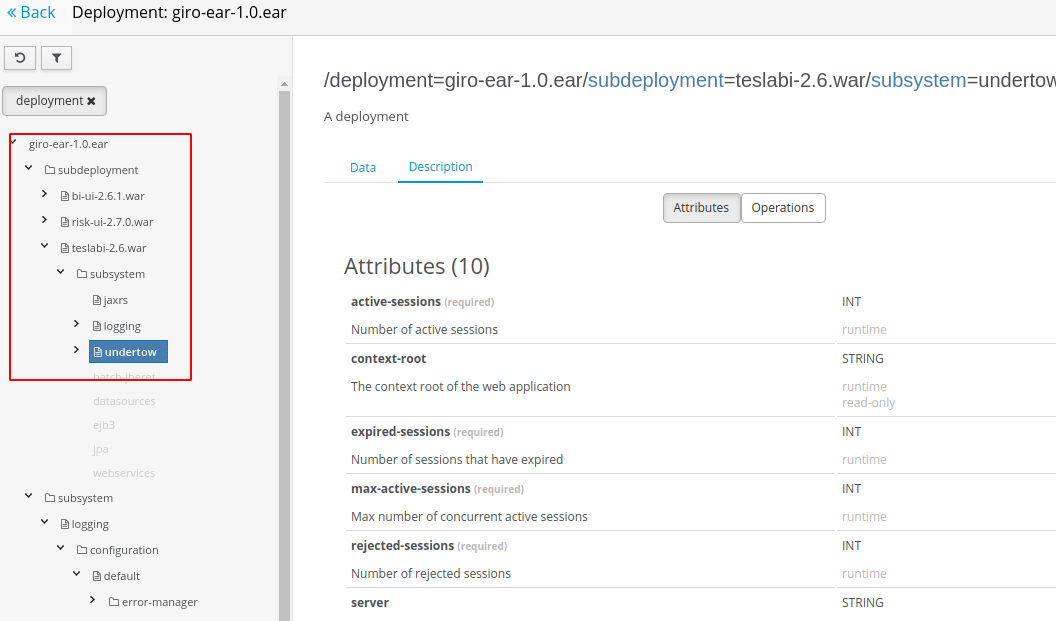
\includegraphics[width=1 \textwidth]{saiku_5}
				\caption {\centering \small{GiroSuite y Rubik-report desplegado en Wilfly 10.1}} \label{figure:chaperIII_7}
				\small {Fuente: \'{A}rea de desarrollo de Tesla Technologies S.A.C, 2018}
			\end{figure}
			
			\item El archivo application.xml fue modificado para contener los artefactos de rubik-report.
			\item Se debe verificar la configuraci\'{o}n de Apache Jack Rabbit para el manejo de archivos y persistencia de los reportes pre-configurados.
		\end{itemize}
		
			
		\subsubsection{Verificar y corregir las librerias de conflicto para las especificaciones del servidor WebLogic 12c + y los archivos weblogic.xml y build.properties}
		\subsubsection{Verificar y corregir librerias de conflicto para las especificaciones del servidor WebSphere 8.0+ y los archivos ibm-web-bnd.xml, ibm-web-ext.xml, deployment.xml y build.properties}
		\subsubsection{La session del usuario administrada por spring security cambiar para que pueda estar centralizada en la base de datos.}
		\subsubsection{Modificar la configuración para la cache de mondrian para tener persistencia con Redis o una base de datos relacional.}
	\subsection{\textit{Sprint Retrospective}}
	
	\subsection{\textit{Increment}}
\end{spacing}